\subsubsection{Total number of messages sent}\label{subsubsec:rect2krmessages}

This is an indication of the energy efficiency of the entire network.

The maximum number of copies is the dominant factor (\(84.89\%\)), as in the
other cases. As in the low density configuration the second most important
factor is the broadcast radius (\(5.58\%\)), with other factors and combinations
that had a negligible influence. The unexplained variation is extremely low
\(0.31\%\).

From \figref{fig:rectperfmessagesR} we notice that also increasing the broadcast
radius is useful to reduce the total number of messages sent when the maximum
number of copies is low, for the same reasons of the last scenario.

\begin{figure}[htb]
	\centering
	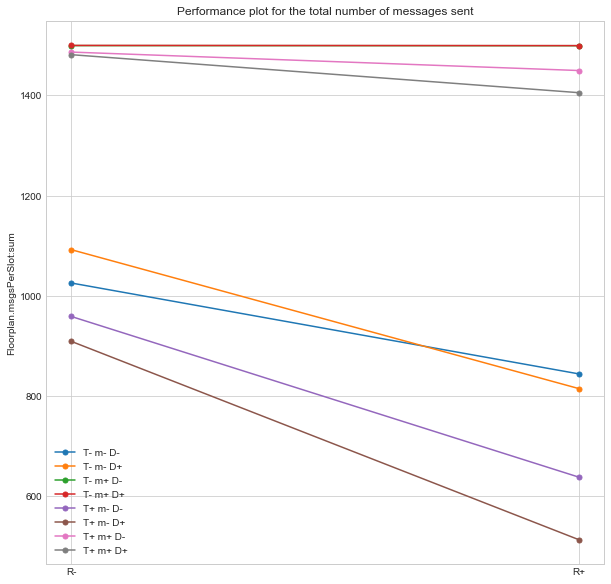
\includegraphics[width=\textwidth]{img/rect/messages_R_perfplot.png}
	\caption{Performance plot for the total number of messages sent. The
	broadcast radius can be used to reduce the total number of messages sent
	when the maximum number of copies is not
	high}\label{fig:rectperfmessagesR}
\end{figure}
